
\chapter{Modeling} \label{ch:modeling}

In order to choose the methods best suited for solving the problems presented in \chapref{ch:intro} a representative model of the system used in this project is needed. This model must thus contain all the physical phenomena which is needed to facilitate methods for solving the presented problems. These phenomena are contact surface pressure responses from the object's texture and topology to the manipulator and frictions between the object and manipulator. Modeling these is done by applying contact and friction models respectively. \medskip

To model the contact for a single contact point can be seen in \figref{fig:model-side-point}. Here the object causes the normal force $\mathbf{f}_N$ at contact point $\mathbf{c}_1$. Once a greater surface are


\begin{center}
    \renewcommand{\arraystretch}{1.2}
    \begin{minipage}{.48\linewidth}
        \vspace{0pt}
        \centering
        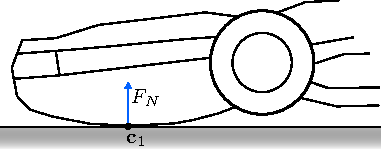
\includegraphics[width=.95\textwidth]{chapters/modeling/fig/side_distribution_schematic-single.pdf}
    \end{minipage}%
    \hfill%
    \begin{minipage}{.48\linewidth}
        \vspace{0pt}
        \centering
        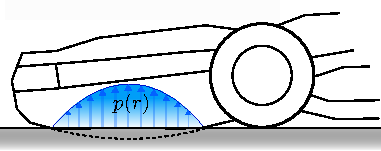
\includegraphics[width=.95\textwidth]{chapters/modeling/fig/side_distribution_schematic-2.pdf}
    \end{minipage}%
    %    
    \vspace{15pt}
    %
    \begin{minipage}[t]{.48\linewidth}
        \vspace{0pt}
        \captionsetup{type=figure}
        \captionof{figure}{Single point of contact between compliant manipulator surface and object surface.}
        \label{fig:model-side-point}
    \end{minipage}%
    \hfill%
    \begin{minipage}[t]{.48\linewidth}
        \vspace{0pt}
        \captionsetup{type=figure}
        \captionof{figure}{Average planning time for each of the interpolation-based trajectory generation methods.}
        \label{fig:model-side-surface}
    \end{minipage}%
\end{center}

Friction models to prevent 


\begin{minipage}{0.45\textwidth}
	\begin{figure}[H]
		\begin{small}
			\begin{center}
				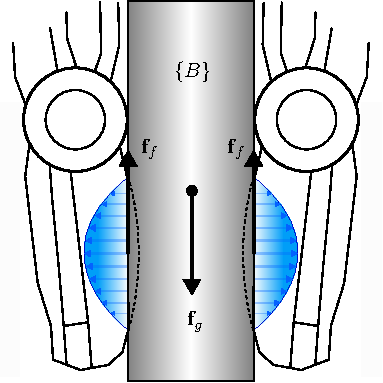
\includegraphics[width=0.95\textwidth]{chapters/modeling/fig/friction_schematic-crop.pdf}
			\end{center}
			\caption{Schematic of Shadow Dexterous Hand from Shadow Robots, based on \cite{shadow-dex-hand-schematic}. The measurements are in \SI{}{\milli\metre}.}
			\label{fig:shadow-dex-hand-schematic}
		\end{small}
	\end{figure}
\end{minipage}



